\documentclass{standalone}

\usepackage[T1]{fontenc}
\usepackage[utf8]{inputenc}
\usepackage{eulervm}
\usepackage{amsmath}
\usepackage{bm}
\usepackage{tikz}
\usepackage{environ}

\usetikzlibrary{fit}
\usetikzlibrary{patterns}
\usetikzlibrary{arrows}

\usepackage{color}

\definecolor{Comment}{RGB}{97,161,176}

\definecolor{btfGreen}{RGB}{51,160,44}
\definecolor{btfRed}{RGB}{190,60,90}

\definecolor{bleuUni}{RGB}{0, 157, 224}
\definecolor{marronUni}{RGB}{68, 58, 49}
\definecolor{grayMarronUni}{RGB}{60, 60, 60}
\definecolor{grayBleuUni}{RGB}{118, 118, 118}

\definecolor{bluecite}{HTML}{009DE0}

\definecolor{Paired-2}{RGB}{166,206,227}
\definecolor{Paired-1}{RGB}{31,120,180}
\definecolor{Paired-4}{RGB}{178,223,138}
\definecolor{Paired-3}{RGB}{51,160,44}
\definecolor{Paired-6}{RGB}{251,154,153}
\definecolor{Paired-5}{RGB}{227,26,28}
\definecolor{Paired-8}{RGB}{253,191,111}
\definecolor{Paired-7}{RGB}{255,127,0}
\definecolor{Paired-10}{RGB}{202,178,214}
\definecolor{Paired-9}{RGB}{106,61,154}
\definecolor{Paired-12}{RGB}{255,255,153}
\definecolor{Paired-11}{RGB}{177,89,40}
\definecolor{Accent-1}{RGB}{127,201,127}
\definecolor{Accent-2}{RGB}{190,174,212}
\definecolor{Accent-3}{RGB}{253,192,134}
\definecolor{Accent-4}{RGB}{255,255,153}
\definecolor{Accent-5}{RGB}{56,108,176}
\definecolor{Accent-6}{RGB}{240,2,127}
\definecolor{Accent-7}{RGB}{191,91,23}
\definecolor{Accent-8}{RGB}{102,102,102}
\definecolor{Spectral-1}{RGB}{158,1,66}
\definecolor{Spectral-2}{RGB}{213,62,79}
\definecolor{Spectral-3}{RGB}{244,109,67}
\definecolor{Spectral-4}{RGB}{253,174,97}
\definecolor{Spectral-5}{RGB}{254,224,139}
\definecolor{Spectral-6}{RGB}{255,255,191}
\definecolor{Spectral-7}{RGB}{230,245,152}
\definecolor{Spectral-8}{RGB}{171,221,164}
\definecolor{Spectral-9}{RGB}{102,194,165}
\definecolor{Spectral-10}{RGB}{50,136,189}
\definecolor{Spectral-11}{RGB}{94,79,162}
\definecolor{Set1-1}{RGB}{228,26,28}
\definecolor{Set1-2}{RGB}{55,126,184}
\definecolor{Set1-3}{RGB}{77,175,74}
\definecolor{Set1-4}{RGB}{152,78,163}
\definecolor{Set1-5}{RGB}{255,127,0}
\definecolor{Set1-6}{RGB}{255,255,51}
\definecolor{Set1-7}{RGB}{166,86,40}
\definecolor{Set1-8}{RGB}{247,129,191}
\definecolor{Set1-9}{RGB}{153,153,153}
\definecolor{Set2-1}{RGB}{102,194,165}
\definecolor{Set2-2}{RGB}{252,141,98}
\definecolor{Set2-3}{RGB}{141,160,203}
\definecolor{Set2-4}{RGB}{231,138,195}
\definecolor{Set2-5}{RGB}{166,216,84}
\definecolor{Set2-6}{RGB}{255,217,47}
\definecolor{Set2-7}{RGB}{229,196,148}
\definecolor{Set2-8}{RGB}{179,179,179}
\definecolor{Dark2-1}{RGB}{27,158,119}
\definecolor{Dark2-2}{RGB}{217,95,2}
\definecolor{Dark2-3}{RGB}{117,112,179}
\definecolor{Dark2-4}{RGB}{231,41,138}
\definecolor{Dark2-5}{RGB}{102,166,30}
\definecolor{Dark2-6}{RGB}{230,171,2}
\definecolor{Dark2-7}{RGB}{166,118,29}
\definecolor{Dark2-8}{RGB}{102,102,102}
\definecolor{Reds-1}{RGB}{255,245,240}
\definecolor{Reds-2}{RGB}{254,224,210}
\definecolor{Reds-3}{RGB}{252,187,161}
\definecolor{Reds-4}{RGB}{252,146,114}
\definecolor{Reds-5}{RGB}{251,106,74}
\definecolor{Reds-6}{RGB}{239,59,44}
\definecolor{Reds-7}{RGB}{203,24,29}
\definecolor{Reds-8}{RGB}{165,15,21}
\definecolor{Reds-9}{RGB}{103,0,13}
\definecolor{Greens-1}{RGB}{247,252,245}
\definecolor{Greens-2}{RGB}{229,245,224}
\definecolor{Greens-3}{RGB}{199,233,192}
\definecolor{Greens-4}{RGB}{161,217,155}
\definecolor{Greens-5}{RGB}{116,196,118}
\definecolor{Greens-6}{RGB}{65,171,93}
\definecolor{Greens-7}{RGB}{35,139,69}
\definecolor{Greens-8}{RGB}{0,109,44}
\definecolor{Greens-9}{RGB}{0,68,27}
\definecolor{Blues-1}{RGB}{247,251,255}
\definecolor{Blues-2}{RGB}{222,235,247}
\definecolor{Blues-3}{RGB}{198,219,239}
\definecolor{Blues-4}{RGB}{158,202,225}
\definecolor{Blues-5}{RGB}{107,174,214}
\definecolor{Blues-6}{RGB}{66,146,198}
\definecolor{Blues-7}{RGB}{33,113,181}
\definecolor{Blues-8}{RGB}{8,81,156}
\definecolor{Blues-9}{RGB}{8,48,107}


\begin{document}
  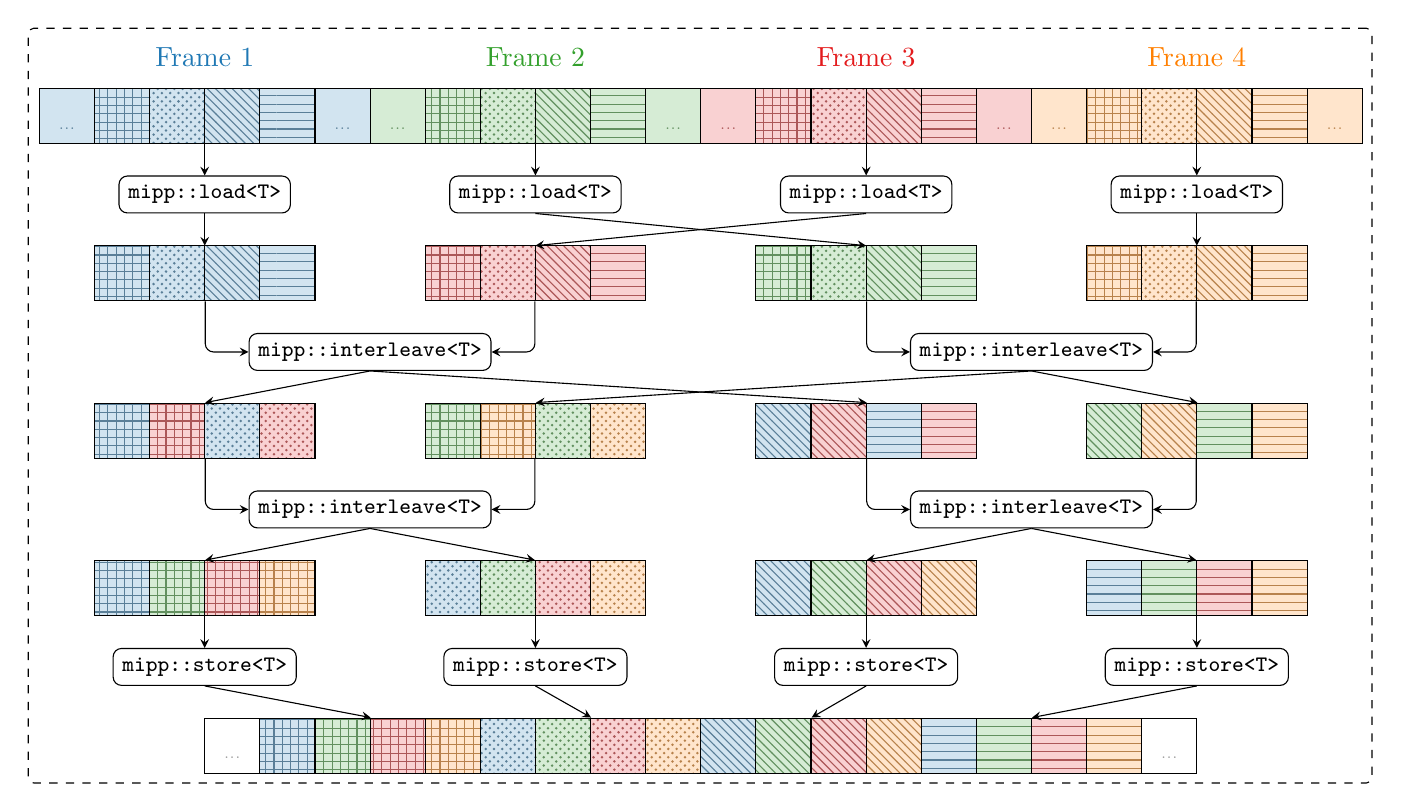
\begin{tikzpicture}[baseline]
    \tikzset{ e1_f1/.style ={draw=black, minimum width=0.7cm, minimum height=0.7cm, text=black, preaction={fill=Paired-1!20}, pattern=grid,             pattern color=black!40!Paired-1!70} }
    \tikzset{ e2_f1/.style ={draw=black, minimum width=0.7cm, minimum height=0.7cm, text=black, preaction={fill=Paired-1!20}, pattern=crosshatch dots,  pattern color=black!40!Paired-1!70} }
    \tikzset{ e3_f1/.style ={draw=black, minimum width=0.7cm, minimum height=0.7cm, text=black, preaction={fill=Paired-1!20}, pattern=north west lines, pattern color=black!40!Paired-1!70} }
    \tikzset{ e4_f1/.style ={draw=black, minimum width=0.7cm, minimum height=0.7cm, text=black, preaction={fill=Paired-1!20}, pattern=horizontal lines, pattern color=black!40!Paired-1!70} }
    \tikzset{ ex_f1/.style ={draw=black, minimum width=0.7cm, minimum height=0.7cm, text=black, fill=Paired-1!20, label={[black!40!Paired-1!70,yshift=-0.65cm]above:\tiny{...}}           } }

    \tikzset{ e1_f2/.style ={draw=black, minimum width=0.7cm, minimum height=0.7cm, text=black, preaction={fill=Paired-3!20}, pattern=grid,             pattern color=black!40!Paired-3!70} }
    \tikzset{ e2_f2/.style ={draw=black, minimum width=0.7cm, minimum height=0.7cm, text=black, preaction={fill=Paired-3!20}, pattern=crosshatch dots,  pattern color=black!40!Paired-3!70} }
    \tikzset{ e3_f2/.style ={draw=black, minimum width=0.7cm, minimum height=0.7cm, text=black, preaction={fill=Paired-3!20}, pattern=north west lines, pattern color=black!40!Paired-3!70} }
    \tikzset{ e4_f2/.style ={draw=black, minimum width=0.7cm, minimum height=0.7cm, text=black, preaction={fill=Paired-3!20}, pattern=horizontal lines, pattern color=black!40!Paired-3!70} }
    \tikzset{ ex_f2/.style ={draw=black, minimum width=0.7cm, minimum height=0.7cm, text=black, fill=Paired-3!20, label={[black!40!Paired-3!70,yshift=-0.65cm]above:\tiny{...}}           } }

    \tikzset{ e1_f3/.style ={draw=black, minimum width=0.7cm, minimum height=0.7cm, text=black, preaction={fill=Paired-5!20}, pattern=grid,             pattern color=black!40!Paired-5!70} }
    \tikzset{ e2_f3/.style ={draw=black, minimum width=0.7cm, minimum height=0.7cm, text=black, preaction={fill=Paired-5!20}, pattern=crosshatch dots,  pattern color=black!40!Paired-5!70} }
    \tikzset{ e3_f3/.style ={draw=black, minimum width=0.7cm, minimum height=0.7cm, text=black, preaction={fill=Paired-5!20}, pattern=north west lines, pattern color=black!40!Paired-5!70} }
    \tikzset{ e4_f3/.style ={draw=black, minimum width=0.7cm, minimum height=0.7cm, text=black, preaction={fill=Paired-5!20}, pattern=horizontal lines, pattern color=black!40!Paired-5!70} }
    \tikzset{ ex_f3/.style ={draw=black, minimum width=0.7cm, minimum height=0.7cm, text=black, fill=Paired-5!20, label={[black!40!Paired-5!70,yshift=-0.65cm]above:\tiny{...}}           } }

    \tikzset{ e1_f4/.style ={draw=black, minimum width=0.7cm, minimum height=0.7cm, text=black, preaction={fill=Paired-7!20}, pattern=grid,             pattern color=black!40!Paired-7!70} }
    \tikzset{ e2_f4/.style ={draw=black, minimum width=0.7cm, minimum height=0.7cm, text=black, preaction={fill=Paired-7!20}, pattern=crosshatch dots,  pattern color=black!40!Paired-7!70} }
    \tikzset{ e3_f4/.style ={draw=black, minimum width=0.7cm, minimum height=0.7cm, text=black, preaction={fill=Paired-7!20}, pattern=north west lines, pattern color=black!40!Paired-7!70} }
    \tikzset{ e4_f4/.style ={draw=black, minimum width=0.7cm, minimum height=0.7cm, text=black, preaction={fill=Paired-7!20}, pattern=horizontal lines, pattern color=black!40!Paired-7!70} }
    \tikzset{ ex_f4/.style ={draw=black, minimum width=0.7cm, minimum height=0.7cm, text=black, fill=Paired-7!20, label={[black!40!Paired-7!70,yshift=-0.65cm]above:\tiny{...}}           } }

    \tikzset{ ex_fx/.style ={draw=black, minimum width=0.7cm, minimum height=0.7cm, text=black, fill=white, label={[black!40,yshift=-0.65cm]above:\tiny{...}}           } }

    \tikzstyle{lnk}=[->,>=stealth,rounded corners=3pt]
    \tikzstyle{shf}=[black!20]
    \tikzstyle{intr}=[rounded corners=3pt, fill=white, draw=black]

    \newcommand\vs{2.0}

    \node[ex_f1] (mi_er0)  at ( 0.0, 0.00) {};
    \node[e1_f1] (mi_er1)  at ( 0.7, 0.00) {};
    \node[e2_f1] (mi_er2)  at ( 1.4, 0.00) {};
    \node[e3_f1] (mi_er3)  at ( 2.1, 0.00) {};
    \node[e4_f1] (mi_er4)  at ( 2.8, 0.00) {};
    \node[ex_f1] (mi_er5)  at ( 3.5, 0.00) {};

    \node[ex_f2] (mi_er6)  at ( 4.2, 0.00) {};
    \node[e1_f2] (mi_er7)  at ( 4.9, 0.00) {};
    \node[e2_f2] (mi_er8)  at ( 5.6, 0.00) {};
    \node[e3_f2] (mi_er9)  at ( 6.3, 0.00) {};
    \node[e4_f2] (mi_er10) at ( 7.0, 0.00) {};
    \node[ex_f2] (mi_er11) at ( 7.7, 0.00) {};

    \node[ex_f3] (mi_er12) at ( 8.4, 0.00) {};
    \node[e1_f3] (mi_er13) at ( 9.1, 0.00) {};
    \node[e2_f3] (mi_er14) at ( 9.8, 0.00) {};
    \node[e3_f3] (mi_er15) at (10.5, 0.00) {};
    \node[e4_f3] (mi_er16) at (11.2, 0.00) {};
    \node[ex_f3] (mi_er17) at (11.9, 0.00) {};

    \node[ex_f4] (mi_er18) at (12.6, 0.00) {};
    \node[e1_f4] (mi_er19) at (13.3, 0.00) {};
    \node[e2_f4] (mi_er20) at (14.0, 0.00) {};
    \node[e3_f4] (mi_er21) at (14.7, 0.00) {};
    \node[e4_f4] (mi_er22) at (15.4, 0.00) {};
    \node[ex_f4] (mi_er23) at (16.1, 0.00) {};

    \node[text width=4cm, text centered, text=Paired-1] (in_f1) at (01.4+0.35, 0.75) {Frame $1$};
    \node[text width=4cm, text centered, text=Paired-3] (in_f2) at (05.6+0.35, 0.75) {Frame $2$};
    \node[text width=4cm, text centered, text=Paired-5] (in_f3) at (09.8+0.35, 0.75) {Frame $3$};
    \node[text width=4cm, text centered, text=Paired-7] (in_f4) at (14.0+0.35, 0.75) {Frame $4$};


    \node[intr] (intr0) at (01.4+0.35, -\vs+1) {\footnotesize{\texttt{mipp::load<T>}}};
    \node[intr] (intr1) at (05.6+0.35, -\vs+1) {\footnotesize{\texttt{mipp::load<T>}}};
    \node[intr] (intr2) at (09.8+0.35, -\vs+1) {\footnotesize{\texttt{mipp::load<T>}}};
    \node[intr] (intr3) at (14.0+0.35, -\vs+1) {\footnotesize{\texttt{mipp::load<T>}}};

    \draw[lnk] (01.4+0.35,-0.35) -- (intr0);
    \draw[lnk] (05.6+0.35,-0.35) -- (intr1);
    \draw[lnk] (09.8+0.35,-0.35) -- (intr2);
    \draw[lnk] (14.0+0.35,-0.35) -- (intr3);

    \node[e1_f1] (r0_er0) at ( 0.7, -\vs) {};
    \node[e2_f1] (r0_er1) at ( 1.4, -\vs) {};
    \node[e3_f1] (r0_er2) at ( 2.1, -\vs) {};
    \node[e4_f1] (r0_er3) at ( 2.8, -\vs) {};

    \node[e1_f3] (r1_er0) at ( 4.9, -\vs) {};
    \node[e2_f3] (r1_er1) at ( 5.6, -\vs) {};
    \node[e3_f3] (r1_er2) at ( 6.3, -\vs) {};
    \node[e4_f3] (r1_er3) at ( 7.0, -\vs) {};

    \node[e1_f2] (r2_er0) at ( 9.1, -\vs) {};
    \node[e2_f2] (r2_er1) at ( 9.8, -\vs) {};
    \node[e3_f2] (r2_er2) at (10.5, -\vs) {};
    \node[e4_f2] (r2_er3) at (11.2, -\vs) {};

    \node[e1_f4] (r3_er0) at (13.3, -\vs) {};
    \node[e2_f4] (r3_er1) at (14.0, -\vs) {};
    \node[e3_f4] (r3_er2) at (14.7, -\vs) {};
    \node[e4_f4] (r3_er3) at (15.4, -\vs) {};

    \draw[lnk] (intr0.south) -- (01.4+0.35,+0.35-\vs);
    \draw[lnk] (intr2.south) -- (05.6+0.35,+0.35-\vs);
    \draw[lnk] (intr1.south) -- (09.8+0.35,+0.35-\vs);
    \draw[lnk] (intr3.south) -- (14.0+0.35,+0.35-\vs);

    \node[intr] (intr4) at (04.2-0.35, -\vs-\vs+1) {\footnotesize{\texttt{mipp::interleave<T>}}};
    \node[intr] (intr5) at (12.6-0.35, -\vs-\vs+1) {\footnotesize{\texttt{mipp::interleave<T>}}};

    \draw[lnk] (r0_er1.south east) |- (intr4.west);
    \draw[lnk] (r1_er2.south west) |- (intr4.east);

    \draw[lnk] (r2_er1.south east) |- (intr5.west);
    \draw[lnk] (r3_er2.south west) |- (intr5.east);

    \node[e1_f1] (r4_er0) at ( 0.7, -\vs-\vs) {};
    \node[e1_f3] (r4_er1) at ( 1.4, -\vs-\vs) {};
    \node[e2_f1] (r4_er2) at ( 2.1, -\vs-\vs) {};
    \node[e2_f3] (r4_er3) at ( 2.8, -\vs-\vs) {};

    \node[e3_f1] (r5_er0) at ( 9.1, -\vs-\vs) {};
    \node[e3_f3] (r5_er1) at ( 9.8, -\vs-\vs) {};
    \node[e4_f1] (r5_er2) at (10.5, -\vs-\vs) {};
    \node[e4_f3] (r5_er3) at (11.2, -\vs-\vs) {};

    \node[e1_f2] (r6_er0) at ( 4.9, -\vs-\vs) {};
    \node[e1_f4] (r6_er1) at ( 5.6, -\vs-\vs) {};
    \node[e2_f2] (r6_er2) at ( 6.3, -\vs-\vs) {};
    \node[e2_f4] (r6_er3) at ( 7.0, -\vs-\vs) {};

    \node[e3_f2] (r7_er0) at (13.3, -\vs-\vs) {};
    \node[e3_f4] (r7_er1) at (14.0, -\vs-\vs) {};
    \node[e4_f2] (r7_er2) at (14.7, -\vs-\vs) {};
    \node[e4_f4] (r7_er3) at (15.4, -\vs-\vs) {};

    \draw[lnk] (intr4.south) -- (r4_er1.north east);
    \draw[lnk] (intr4.south) -- (r5_er1.north east);

    \draw[lnk] (intr5.south) -- (r6_er1.north east);
    \draw[lnk] (intr5.south) -- (r7_er1.north east);

    \node[intr] (intr6) at (04.2-0.35, -\vs-\vs-\vs+1) {\footnotesize{\texttt{mipp::interleave<T>}}};
    \node[intr] (intr7) at (12.6-0.35, -\vs-\vs-\vs+1) {\footnotesize{\texttt{mipp::interleave<T>}}};

    \draw[lnk] (r4_er1.south east) |- (intr6.west);
    \draw[lnk] (r6_er2.south west) |- (intr6.east);

    \draw[lnk] (r5_er1.south east) |- (intr7.west);
    \draw[lnk] (r7_er2.south west) |- (intr7.east);

    \node[e1_f1] (r8_er0) at ( 0.7, -\vs-\vs-\vs) {};
    \node[e1_f2] (r8_er1) at ( 1.4, -\vs-\vs-\vs) {};
    \node[e1_f3] (r8_er2) at ( 2.1, -\vs-\vs-\vs) {};
    \node[e1_f4] (r8_er3) at ( 2.8, -\vs-\vs-\vs) {};

    \node[e2_f1] (r9_er0) at ( 4.9, -\vs-\vs-\vs) {};
    \node[e2_f2] (r9_er1) at ( 5.6, -\vs-\vs-\vs) {};
    \node[e2_f3] (r9_er2) at ( 6.3, -\vs-\vs-\vs) {};
    \node[e2_f4] (r9_er3) at ( 7.0, -\vs-\vs-\vs) {};

    \node[e3_f1] (r10_er0) at ( 9.1, -\vs-\vs-\vs) {};
    \node[e3_f2] (r10_er1) at ( 9.8, -\vs-\vs-\vs) {};
    \node[e3_f3] (r10_er2) at (10.5, -\vs-\vs-\vs) {};
    \node[e3_f4] (r10_er3) at (11.2, -\vs-\vs-\vs) {};

    \node[e4_f1] (r11_er0) at (13.3, -\vs-\vs-\vs) {};
    \node[e4_f2] (r11_er1) at (14.0, -\vs-\vs-\vs) {};
    \node[e4_f3] (r11_er2) at (14.7, -\vs-\vs-\vs) {};
    \node[e4_f4] (r11_er3) at (15.4, -\vs-\vs-\vs) {};

    \draw[lnk] (intr6.south) -- (r8_er1.north east);
    \draw[lnk] (intr6.south) -- (r9_er2.north west);

    \draw[lnk] (intr7.south) -- (r10_er1.north east);
    \draw[lnk] (intr7.south) -- (r11_er2.north west);

    \node[intr] (intr8)  at (01.4+0.35, -\vs-\vs-\vs-\vs+1) {\footnotesize{\texttt{mipp::store<T>}}};
    \node[intr] (intr9)  at (05.6+0.35, -\vs-\vs-\vs-\vs+1) {\footnotesize{\texttt{mipp::store<T>}}};
    \node[intr] (intr10) at (09.8+0.35, -\vs-\vs-\vs-\vs+1) {\footnotesize{\texttt{mipp::store<T>}}};
    \node[intr] (intr11) at (14.0+0.35, -\vs-\vs-\vs-\vs+1) {\footnotesize{\texttt{mipp::store<T>}}};

    \draw[lnk] (01.4+0.35,-\vs-\vs-\vs-0.35) -- (intr8);
    \draw[lnk] (05.6+0.35,-\vs-\vs-\vs-0.35) -- (intr9);
    \draw[lnk] (09.8+0.35,-\vs-\vs-\vs-0.35) -- (intr10);
    \draw[lnk] (14.0+0.35,-\vs-\vs-\vs-0.35) -- (intr11);


    \node[ex_fx] (mo_er0)  at ( 2.1, -\vs-\vs-\vs-\vs+0.00) {};
    \node[e1_f1] (mo_er1)  at ( 2.8, -\vs-\vs-\vs-\vs+0.00) {};
    \node[e1_f2] (mo_er2)  at ( 3.5, -\vs-\vs-\vs-\vs+0.00) {};
    \node[e1_f3] (mo_er3)  at ( 4.2, -\vs-\vs-\vs-\vs+0.00) {};
    \node[e1_f4] (mo_er4)  at ( 4.9, -\vs-\vs-\vs-\vs+0.00) {};
    \node[e2_f1] (mo_er5)  at ( 5.6, -\vs-\vs-\vs-\vs+0.00) {};
    \node[e2_f2] (mo_er6)  at ( 6.3, -\vs-\vs-\vs-\vs+0.00) {};
    \node[e2_f3] (mo_er7)  at ( 7.0, -\vs-\vs-\vs-\vs+0.00) {};
    \node[e2_f4] (mo_er8)  at ( 7.7, -\vs-\vs-\vs-\vs+0.00) {};
    \node[e3_f1] (mo_er9)  at ( 8.4, -\vs-\vs-\vs-\vs+0.00) {};
    \node[e3_f2] (mo_er10) at ( 9.1, -\vs-\vs-\vs-\vs+0.00) {};
    \node[e3_f3] (mo_er11) at ( 9.8, -\vs-\vs-\vs-\vs+0.00) {};
    \node[e3_f4] (mo_er12) at (10.5, -\vs-\vs-\vs-\vs+0.00) {};
    \node[e4_f1] (mo_er13) at (11.2, -\vs-\vs-\vs-\vs+0.00) {};
    \node[e4_f2] (mo_er14) at (11.9, -\vs-\vs-\vs-\vs+0.00) {};
    \node[e4_f3] (mo_er15) at (12.6, -\vs-\vs-\vs-\vs+0.00) {};
    \node[e4_f4] (mo_er16) at (13.3, -\vs-\vs-\vs-\vs+0.00) {};
    \node[ex_fx] (mo_er17) at (14.0, -\vs-\vs-\vs-\vs+0.00) {};

    \draw[lnk] (intr8.south)  -- (mo_er2.north east);
    \draw[lnk] (intr9.south)  -- (mo_er6.north east);
    \draw[lnk] (intr10.south) -- (mo_er10.north east);
    \draw[lnk] (intr11.south) -- (mo_er14.north east);

    \node[draw=black, rounded corners=2pt, dashed, fit=(mi_er0) (mi_er23) (in_f1) (mo_er0)] {};

  \end{tikzpicture}
\end{document}